%%%%%%
%
% $Autor: Wings $
% $Datum: 2020-01-18 11:15:45Z $
% $Pfad: WuSt/Skript/Produktspezifikation/powerpoint/ImageProcessing.tex $
% $Version: 4620 $
%
%%%%%%

% 
%todo  \url{http://www.industry-analytics.de/ki-wann-sind-maschinen-intelligent/}




\chapter{Artificial intelligence - When are machines intelligent?}

Answering the question is not easy. First, the term intelligence must be defined. Its definition is not unambiguous.  For example, it is not defined at what point a person is considered intelligent. This raises the question of what belongs to intelligence. In psychology, intelligence includes, among other things, the ability to adapt to unknown and situations, but also to solve new problems.\cite{Funke:1998}


\section{What is Artificial Intelligence?}

Consequently, the term artificial intelligence is also not clearly defined. Historically, the term was introduced by John McCarthy  \cite{McCarthy:2006}:

\bigskip

\textsl{\glqq The aim of AI is to develop machines that behave as if they had intelligence.\grqq{}} - John McCarthy, 1955
	
\bigskip

According to this definition, simple machines and sensors are intelligent. They act in accordance with a programme. This means that all reactions of the system have been determined and fixed beforehand. If individual characteristics of humans are considered, then, according to machines, a great many machines can be considered intelligent; especially since machines have taken over activities that are wholly or partially performed by humans. A simple example is computer programs. They are many times more efficient in this area than humans. Hence the following definition \cite{Rich:1983}:


\bigskip

\textsl{\glqq AI is the study of how to make computers do things which, at the moment, people do better.\grqq{}} - Elaine Rich, 1983 

\bigskip

This approach is clever in that it does not circumvent the definition of intelligence. On the other hand, it points out that it is a snapshot in time. This takes into account,
that the human being is very adaptable. This adaptability distinguishes him in particular. Man is able to grasp new external influences and adapt to them. He can
learn independently.

\bigskip

In the decade from 2010 to 202, many impressive results were achieved in the field of artificial intelligence. In 2011, the computer Watson defeated the human champion in the very popular guessing show \glqq Jeopardy\grqq{} \cite{Ferrucci:2012}. Professional players of the board game Go were beaten by System AlphaGo for the first time in 2015 and 2016 \Cite{Wang:2016}. Even bluffing in poker was successfully applied by an artificial intelligence called Libratus in 2017 \cite{Brown:2018}. In 2018, a computer program from the Chinese corporation Alibaba shows better reading comprehension than humans. The software, GPT-3, writes 2020 non-fiction text and poetry that looks like it was created by humans. Artificial intelligences have also become active in the art world; new songs by the Beatles have been composed and paintings created in the style of famous painters. These successes tempt one to conclude that computer software is superior to human intelligence. To clarify the difference, the terms weak and strong intelligence are introduced. Strong artificial intelligence is for all-encompassing software that can adapt to different or new requirements. In contrast, weak artificial intelligence means that an algorithm has been developed to solve a specific task. They can solve complex and demanding tasks from very different fields as well as humans or better. The above list shows that weak AIs deliver stunning results. But strong artificial intelligence does not exist any more than a time machine.
%Time.com/ 2021/13
In the graphic~\ref{figKIMLDL} the relationships between strong, weak Artificial Intelligence, Machine Learning and Deep Learning are shown; according to this, Deep Learning is a subfield of Machine Learning and this in turn is a subfield of Artificial Intelligence.

\begin{figure}
    \begin{center}
        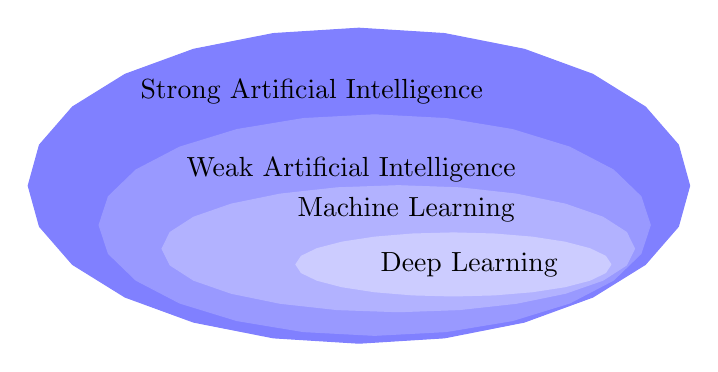
\begin{tikzpicture}
            \draw [blue!50,fill=blue!50,domain=0:360] plot ({-1.2+4.2*cos(\x)}, {0.6+2.0*sin(\x)});
            \draw [blue!40,fill=blue!40,domain=0:360] plot ({-1+3.5*cos(\x)}, {0.1+1.4*sin(\x)});
            \draw [blue!30,fill=blue!30,domain=0:360] plot ({-0.7+3*cos(\x)}, {-0.2+0.8*sin(\x)});
            \draw [blue!20,fill=blue!20,domain=0:360] plot ({2*cos(\x)}, {-0.4+0.4*sin(\x)});
            
            \node (DP) at (0.2,-0.4) {Deep Learning};
            \node (ML) at (-0.6,0.3) {Machine Learning};
            \node (AI) at (-1.3,0.8) {Weak Artificial Intelligence};
            \node (AI) at (-1.8,1.8) {Strong Artificial Intelligence};
        \end{tikzpicture}
        
        \caption{relationship of artificial intelligence, machine learning and deep learning}\label{figKIMLDL}
    \end{center}
\end{figure}


\section{Machinelles Lernen}

Machine learning represents the ability of a machine to extract knowledge from available data and recognise patterns. If necessary, this pattern can then be applied to subsequent data sets. The way in which the learning process takes place can be divided into three categories:

\begin{description}
    \item[Supervised learning] uses training and test data for the learning process. The training data includes both input data (e.g. object metrics) and the desired result (e.g. classification of objects). The algorithm should then use the training data to find a function that maps the input data to the result. Here, the function is adapted independently by the algorithm during the learning process. Once a certain success rate has been achieved for the training data, the learning process is verified with the help of the test data. An example of this would be a clustering procedure in which the clusters are already known before the learning process begins. 
    
    \item[Unsupervised learning] uses only input data for the learning process, where the outcome is not yet known. Based on the characteristics of the input data, patterns are to be recognised in this. One application of unsupervised learning is the clustering of data where the individual clusters are not yet defined before the learning process. 
    
    \item[Reinforcement] learning is based on the reward principle for actions that have taken place. It starts in an initial state without information about the environment or about the effects of actions. An action then leads to a new state and provides a reward (positive or negative). This is done until a final condition occurs. The learning process can then be repeated to maximise the reward. 
\end{description}

\section{Deep Learning}
 
 Deep Learning represents a sub-field of machine learning and uses a \ac{nn} for the learning process. These represent a model of the human brain and the neuronal processes. The \ac{knn} consists of nodes representing neurons. A distinction is made between three categories of neurons. 
 
%\GRAPHICSC{1.0}{1.0}{kdd/Knn}


\begin{figure}
  \begin{center}
    
    \def\layersep{2.5cm}
    
    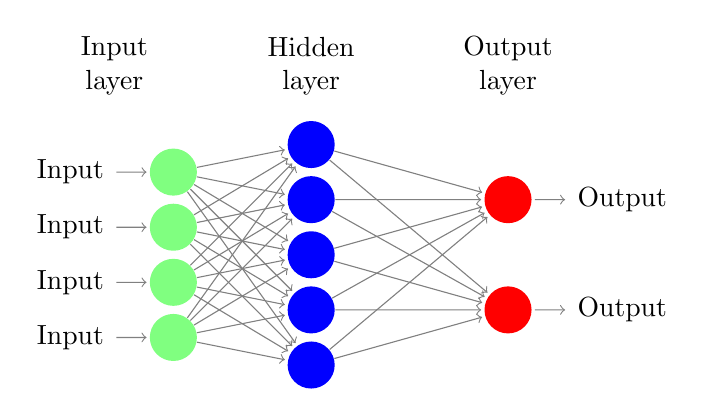
\begin{tikzpicture}[shorten >=1pt,->,draw=black!50, node distance=\layersep,scale=0.7]
      \tikzstyle{every pin edge}=[<-,shorten <=1pt]
      \tikzstyle{neuron}=[circle,fill=black!25,minimum size=17pt,inner sep=0pt]
      \tikzstyle{input neuron}=[neuron, fill=green!50];
      \tikzstyle{output neuron}=[neuron, fill=red];
      \tikzstyle{hidden neuron}=[neuron, fill=blue];
      \tikzstyle{annot} = [text width=4em, text centered]
        
      % Draw the input layer nodes
      \foreach \name / \y in {1,...,4}
        % This is the same as writing \foreach \name / \y in {1/1,2/2,3/3,4/4}
        \node[input neuron, pin=left:Input] (I-\name) at (0,-\y) {};
        
        % Draw the hidden layer nodes
      \foreach \name / \y in {1,...,5}
        \path[yshift=0.5cm]
        node[hidden neuron] (H-\name) at (\layersep,-\y cm) {};
        
        % Draw the output layer node
        \node[output neuron,pin={[pin edge={->}]right:Output}, right of=H-2] (O1) {};
        \node[output neuron,pin={[pin edge={->}]right:Output}, right of=H-4] (O2) {};
        
        % Connect every node in the input layer with every node in the
        % hidden layer.
        \foreach \source in {1,...,4}
          \foreach \dest in {1,...,5}
            \path (I-\source) edge (H-\dest);
        
        % Connect every node in the hidden layer with the output layer
        \foreach \source in {1,...,5}
          \path (H-\source) edge (O1);
        \foreach \source in {1,...,5}
          \path (H-\source) edge (O2);
        
        % Annotate the layers
        \node[annot,above of=H-1, node distance=1cm] (hl) {Hidden layer};
        \node[annot,left of=hl] {Input layer};
        \node[annot,right of=hl] {Output layer};
    \end{tikzpicture}
  \end{center}
  \caption{Example of a \ac{knn}}\label{fig:knn}
\end{figure}


\begin{description}
  \item[input neurons] are the neurons that receive signals from the outside world. Here there is one neuron for each type of input (feature).
\item [hidden neurons] are neurons that represent the actual learning process.
\item [output neurons] are the neurons that give signals to the outside world. There is one neuron for each type of output (feature).
\end{description}

\bigskip

All neurons of a category are combined into a layer. Thus, in each neural network there is an input layer, see figure\ref{fig:knn} green neurons, a hidden layer, in the figure~\ref{fig:knn} the blue neurons, and an output layer with the red neurons in the figure~\ref{fig:knn}. If a \ac{knn} contains more than one hidden layer, it is called a deep neural network. The connections between the neurons in each layer are called synapses. These contain a weighting, which is multiplied by the signal of the start neuron. Thus, the individual signals are weighted. The weights are in turn adjusted during the learning process, based on functions.


\section{Application}

Due to the adaptability of artificial intelligences, they can be used in many different ways. In its study \glqq Smartening up with Artificial Intelligence (AI)\grqq{}, McKinsey described eight application scenarios in which artificial intelligence has particular potential \cite{McKinsey:2017}.

\begin{itemize}
    \item Autonomous Vehicles
    \item Predictive maintenance through better forecasting 
    \item Collaborative robotics with perception of the environment (machine-machine interaction \& human-machine interaction)
    \item Quality improvement through autonomous adaptation of machines to products to be processed
    \item Automated quality inspection
    \ Supply chain management through more accurate forecasting
    \ Research and development
    \item Automated support processes
\end{itemize}


%todo Gedanke industrie 4.0 / Edge-Computer ist gut, sonst raus


%Wenn es einen Bereich gibt, der prägend für das 21. Jahrhundert ist, dann mit Sicherheit
%die Künstliche Intelligenz, die uns heutzutage in vielen Dingen des Alltags begegnet.
%Im privaten Rahmen haben sich beispielsweise persönliche Sprachassistenten, wie zum Beispiel
%Alexa von Amazon, in viele Haushalte integriert. Diese beantworten über Sprachbefehle
%alle Fragen, schalten auf Befehl das Licht an oder spielen die Lieblingsmusik. Im 
%industriellen Umfeld forschen große Automobilbranchen daran, dass autonome Fahren weiter
%voranzubringen und mit Hilfe der künstlichen Intelligenz den Straßenverkehr sicherer zu
%gestalten.
%
%Das Grundprinzip der künstlichen Intelligenz existiert schon seit Ende der 1950er, doch
%hat es erst mit dem technischen Fortschritt in der Computerindustrie und der zunehmenden 
%Vernetzung der Welt sein Potential weiter entfalten können. Die Bundesregierung
%in Deutschland hat großes Interesse daran, die Entwicklung der künstlichen Intelligenz
%schnell voranzutreiben, um weltweit die Wettbewerbsfähig zu sicher und fördert Projekte
%in diesem Bereich mit Milliardenpaketen. \cite{Hubel:1959,Werle:2020} 
%
%Besonders interessant ist diese Technologie für Unternehmen, die sich nach den Grundsätzen
%der \glqq Industrie 4.0\grqq{} weiterentwickeln wollen. Grundlegendes Ziel dabei ist, 
%das Eingreifen des Menschen in den Produktionsprozess zu minimieren und die digitale 
%Kommunikation von Anlagen untereinander zu maximieren. Der Produktionsprozess soll dadurch 
%transparenter gestaltet und optimiert werden. Besonders gut dafür geeignet sind 
%Edge-Computing-Systeme, welche Daten dezentral und in Echtzeit verarbeiten und auswerten 
%können. Die daraus resultierenden Ergebnisse können anschließend an einen zentralen Server 
%weitergeleitet werden. \cite{Martins:2019}
%
%Als Werkzeug zur Steigerung von Effizienz und Effektivität industrieller Prozesse, auch 
%durch einen höheren Autonomiegrad, spielt die künstliche Intelligenz eine wichtige Rolle.
%Im Feld, dem sogenannten Edge-Bereich, können Systeme für künstliche Intelligent
%von jedem durch Systeme wie den Jetson Nano entwickelt und erprobt werden.
%\cite{JetsonProjects:2020}
%
%
%
%
%%\glqq Die Künstliche Intelligenz, kurz KI, einfach erklärt, ist der Versuch, menschliches Lernen und Denken auf den Computer zu übertragen und ihm damit Intelligenz zu verleihen. Statt für jeden Zweck programmiert zu werden, kann eine KI eigenständig Antworten finden und selbstständig Probleme lösen.\grqq{} \cite{KI:2020}
%%
%%\bigskip
%
%
